\section{Substytucja rodnikowa $(S_R)$}

Reakcje substytucji, zwane też reakcjami podstawienia, to reakcje, w których następuje wymiana atomu lub grupy atomów w jednej cząsteczce na inny atom lub grupę atomów z innej cząsteczki.
\newline

W substytucji rodnikowej odczynnikiem atakującym jest rodnik. Rodnikami nazywamy cząsteczki, atomy, a najczęściej fragmenty cząsteczek mające niesparowany elektron.
\newline

Rodniki powstają pod wpływem światła (hv) lub podwyższonej temperatury. Są one bardzo aktywne, gdyż mają niesparowany elektron. 

\subsection{Mechanizm reakcji pod wpływem hv}
\vspace{0.7cm}

\subsubsection{Inicjacja}
\vspace{0.5cm}

\schemestart
    \chemname{\chemfig{Cl_2}}{cząsteczka chloru}
    \arrow{->[hv]}
    \chemfig{Cl^\bullet}
    \+
    \chemname{\chemfig{Cl^\bullet}}{rodnik chloru}
\schemestop

\subsubsection{Propagacja}
\vspace{0.5cm}

\begin{itemize}
    \item[]
\schemestart
    \chemfig{Cl^\bullet}
    \+
    \chemfig{CH_4}
    \arrow{->}
    \chemfig{CH_3^\bullet}
    \+
    \chemfig{HCl}
\schemestop
    \item[]
\vspace{0.5cm}
\schemestart
    \chemfig{CH_3^\bullet}
    \+
    \chemfig{Cl_2}
    \arrow{->}
    \chemfig[atom sep=2em]{CH_3-Cl}
    \+
    \chemfig{Cl^\bullet}
\schemestop

\end{itemize}

\subsubsection{Terminacja}
\vspace{0.5cm}

\begin{itemize}
    \item[]
\schemestart
    \chemfig{2Cl^\bullet}
    \arrow{->}
    \chemfig{Cl_2}
\schemestop
    \item[]
\schemestart
    \chemfig{2CH_3^\bullet}
    \arrow{->}
    \chemfig[atom sep=2em]{CH_3-CH_3}
\schemestop
    \item[]
\schemestart
    \chemfig{Cl^\bullet}
    \+
    \chemfig{CH_3^\bullet}
    \arrow{->}
    \chemname{\chemfig[atom sep=2em]{CH_3-Cl}}{produkt główny}
\schemestop
  
\end{itemize}

\newpage
\subsection{Addycja wolnorodnikowa ($A_R$)}

\begin{figure}[H]
    \centering
    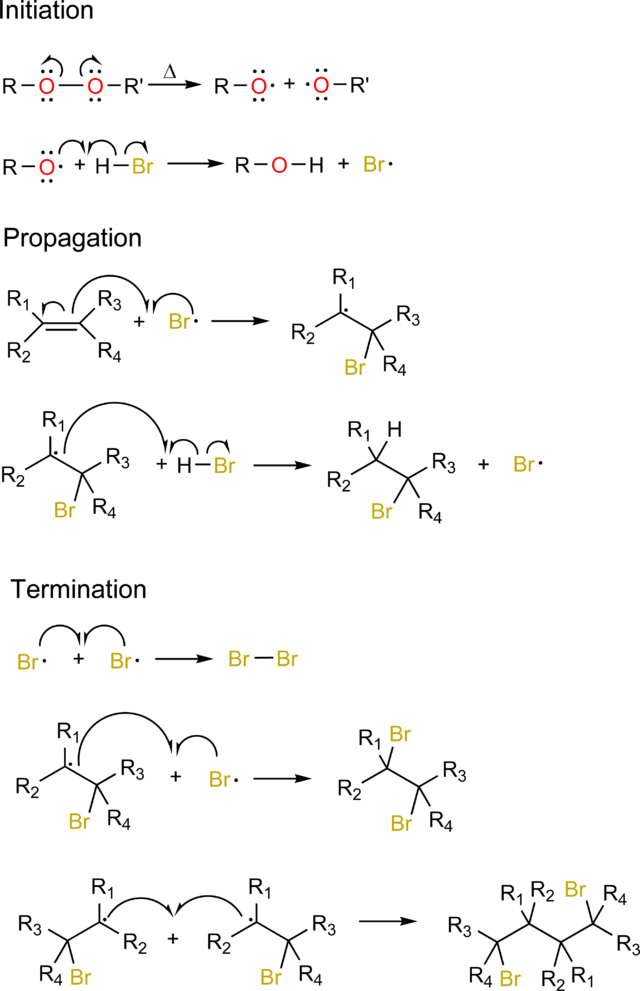
\includegraphics[width=0.7\textwidth]{img/roor}
    \label{fig.roor}
\end{figure}